\chapter{AC Circuits}
\label{15}
\section{Direct Current}
\textit{\textbf{“That type of current that flows in the circuit 
elements in one direction.”}}
It is important to note that the direction of D.C remains constant
but the magnitude is not necessarily constant. On this basis, D.C
can be divided into two types:
\begin{enumerate}
    \item Pure D.C
    \item Pulsating D.C
\end{enumerate}
\subsection{Pure D.C}
\textit{\textbf{“That type of D.C in which neither the direction nor 
the magnitude changes is called pure D.C.”}}   
\newline
e.g. Battery is a source of pure D.C.
\subsubsection{Graphical Representation}
%figure

\subsection{Pulsating D.C}
\textit{\textbf{“That type of D.C whose direction remains same
but magnitude changes is called pulsating D.C.”}} 
\subsubsection{Graphical Representation}
Graphically, pulsating D.C is shown by a wavy line with the passage of
time. It is important to note that voltage or current is positive
all the time i.e. the current direction remains same.

\section{Alternating Current}
\textit{\textbf{“That type of current whose magnitude changes
and direction reverses many times in a second is called
alternating current.”}}
\begin{center}
    OR
\end{center}
\textit{\textbf{“A voltage which changes its polarity at regular
intervals of time is called alternating voltage and current
produced by that voltage is called alternating current.”}}

\subsection*{Explanation}    
When an alternating voltage is applied in a circuit, the current flows
first in one direction and then in the opposite direction, the direction of current at any instant depends upon the polarity of the voltages.
Consider the figure below in which an alternating voltage source is
connected to a resistor ‘$R$’ as shown:
%figure

When the upper terminal of the A.C source is positive and the
lower terminal is negative, the current flows in one direction
shown in figure \ref{fig:15.3}. After half the time period, the polarity of the
voltage source is reversed, the current flows in opposite direction.
Such a current is called alternating current because the current flows
in the alternate directions in the circuit. 
\section{Sinusoidal Alternating Voltage and Current}
\textit{\textbf{“The current which reverses its direction many times 
in a second, is known as alternating current.”}}
 
Sinusoidal means a curve which obeys graph of sine function.
Sinusoidal voltage can be produced by rotating a coil with a
uniform angular velocity. A.C voltage switches polarity over time.
When graphed over time, the “wave” traced by this voltage of alternating
polarity from an alternator takes on a distinct shape, known as sine wave. 

\subsection*{Graphical Demonstration}
The sinusoidal waveform is shown in figure \ref{fig:15.4}.
\begin{figure}[H]
    \centering
    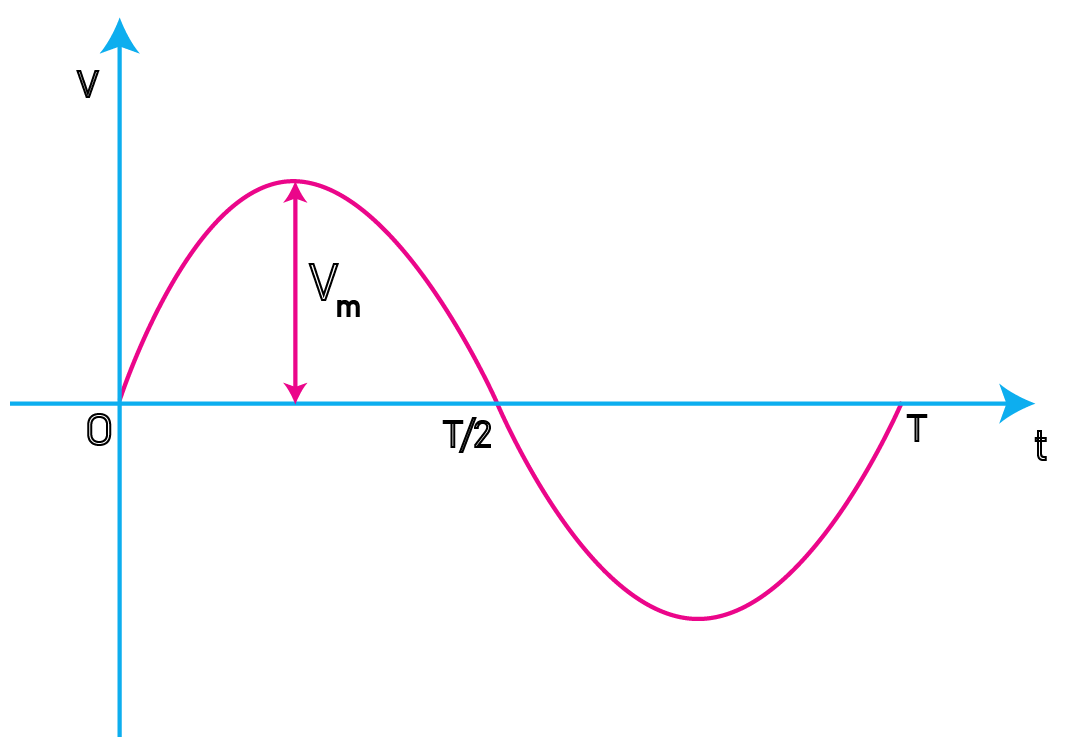
\includegraphics[scale = 0.6]{Images/Chapter-15/15.4}
    \caption{Sinusoidal waveform.}
    \label{fig:15.4}
\end{figure}

\subsection*{Mathematical Form}
The output at any instant of time ‘$t$’ is represented by:
\begin{mybox}{red}{}
\begin{equation}\label{eq:15.1}
    V = V_{m} sin \omega t
\end{equation}
\end{mybox}
\noindent where,
\newline
$V$ = Instantaneous voltage
\newline
$V_{m}$= maximum or peak value or the amplitude of sinusoidal voltage
\newline
$\omega$ = angular frequency of A.C source (rad/s)
\newline
$t$ = time
\newline
Also,
\begin{center}
    $ \omega = 2 \pi f $
\end{center}
So, equation \ref{eq:15.1} implies:
\begin{equation}\label{eq:15.2}
    V = V_{m} sin 2 \pi f t
\end{equation}
Similarly, sinusoidal current can be represented as:
\begin{mybox}{red}{}
\begin{equation}\label{eq:15.3}
    I = I_{m} sin \omega t
\end{equation}
\end{mybox}
\noindent From the figure \ref{fig:15.4}, it is obvious that voltage or current
not only changes direction at regular intervals but the magnitude is
also changing continuously.

\subsection{Average Value of Alternating Voltage and Current}
\textit{\textbf{“The average of the alternating voltage or current over
one cycle is called mean value/average value.”}}
\begin{center}
    OR
\end{center}
\textit{\textbf{“The sum of entire positive and negative values over
one cycle divided by the time period.”}}  

\subsubsection{Explanation}
As the current and voltage is varying sinusoidally, so we should take
average value to measure it, the graph is shown in figure \ref{fig:15.5}.
\begin{figure}[H]
    \centering
    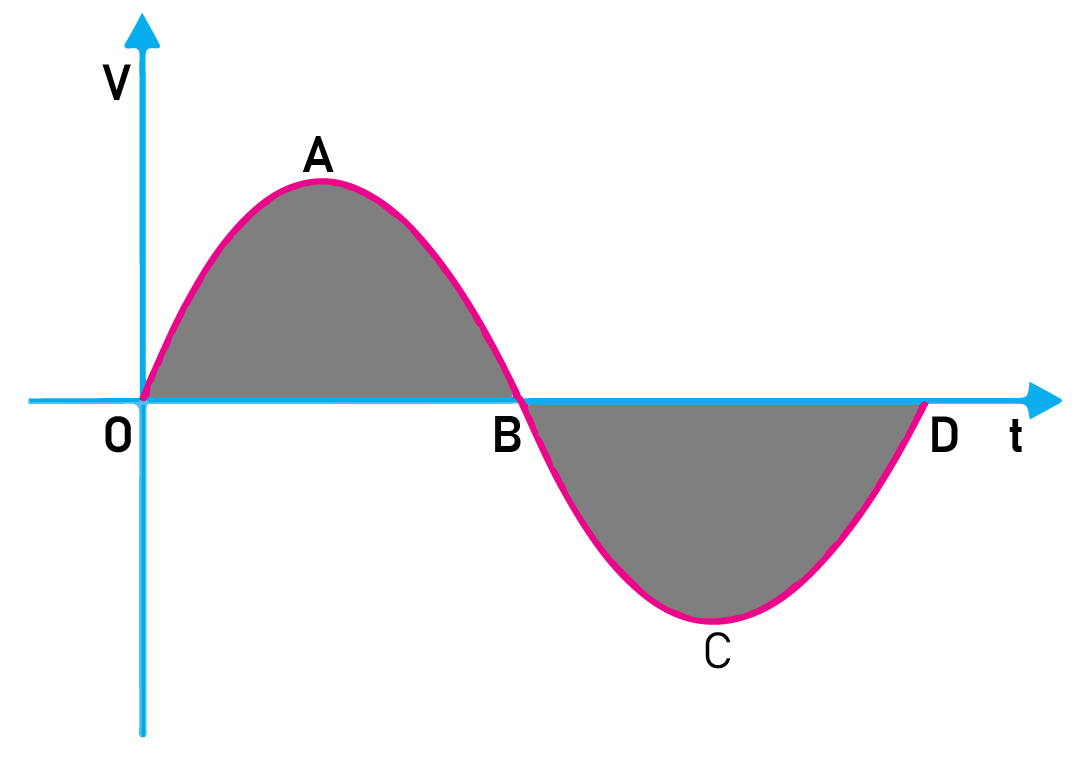
\includegraphics[scale = 0.6]{Images/Chapter-15/15.5}
    \caption{Sinusoidal voltage.}
    \label{fig:15.5}
\end{figure}
To find the average value, we have to add values in the positive as
well as the negative cycle and divided by time for one cycle.
From the graph, it is clear that:
\begin{enumerate}[label = (\roman*)]
    \item The sum of all the positive values in one cycle is the area
    of the upper lobe (shaded region OAB).
    \item The sum of all the negative values is the area of all the
    lower lobe (shaded area BCD).
\end{enumerate}
So,
\begin{equation}
    Mean Value = \frac{Area under OAB - Area under BCD }{Time Period}
\end{equation}
As,
\begin{center}
    Area OAB = Area BCD
\end{center}
Hence, mean value of ‘$V$’ or ‘$I$’ over one cycle is zero.

Using Calculus (average value of a function over an interval [a,b]
by mean value theorem):

\begin{equation}\notag
\begin{split}
    \overline{V}&= \frac{1}{b-a} \int_{a}^{b} sinx\:dx\\
     &= \frac{1}{2\pi-0} \int_{0}^{2\pi} sinx\:dx\\
     &= \frac{1}{2\pi} (cos2 \pi - cos0)\\ 
     &= \frac{1}{2\pi} (1-1)\\
     \overline{V}&=0 
\end{split}
\end{equation}
Same is for I.
\begin{mybox}{green}{}
\subsubsection*{\note{}Note:}This result is valid only for sinusoidal
voltage or current.   
\end{mybox}
\subsection{Root mean square value}
\textit{\textbf{“It is the value of that direct current which would produce heat at the same rate as the alternating current in a given resistor.”}}  

\subsubsection*{Explanation}
As we know that the mean value of alternating current $(<I>)$ or voltage $(<V>)$ is zero over a cycle but practically, a heater operated with alternating current produces heat. If the effective value of current is zero, how would a heater could produce heat. As,
\begin{equation}
    P= I^{2}R = \frac{V^{2}}{R}
\end{equation}
Equation \ref{eq:12.5} uses squares of $I$ and $V$ rather than $I$ and $V$,
so it is obvious that we should find the mean value
of $I\textsuperscript{2}$ and $V\textsuperscript{2}$ rather than $I$
and $V$, which are called mean square values (average values of
the squared quantities).

Consider the figure showing a graph of sinusoidal current and its
squared value $I\textsuperscript{2}$ varying with time $t$.
%figure

From the figure, squared values of positive numbers as well as
negative numbers are positive, therefore the values
of $I^{2}$ are positive for the positive as well as negative half cycle.
As it is known (You can find it by using integral from 0 to $\pi$) that
value of $sin^{2}\omega t$ is $\frac{1}{2}$ in one cycle. So,
\begin{equation}\notag
    <I^{2}> = < I_{0}^{2} sin^{2} \omega t >
\end{equation}
\begin{equation}\notag
    <I^{2}> = \frac{1}{2}  I_{0}^{2} 
\end{equation}
Taking square root on both sides of the equation:
\begin{equation}\notag
   \sqrt{ <I^{2}>} = \frac{I_{0}}{\sqrt{2}}  
\end{equation}
And this value $\sqrt{ <I^{2}>}$ (The root of an average of a square) is
called root mean square value of $I$ and is denoted by 
$I_{rms}$.
Hence, we can write:
\begin{mybox}{red}{}
    \begin{equation}\label{15.6}
        I_{rms} = \frac{I_{0}}{\sqrt{2}}  
     \end{equation}
     \begin{equation}
        I_{rms} = 0.707 I_{0}  
     \end{equation}  
\end{mybox}
\subsubsection{Relation between $I_{dc}$ and $I_{rms}$}
$I_{dc}$ is the effective value of DC which would deliver the same power to a resistor as the AC to the same resistor i.e
\begin{equation}\notag
    P_{dc} = P_{ac}
\end{equation}
And,
\begin{equation}\notag
    P_{dc} = I^{2}R
\end{equation}
\begin{equation}\notag
    P_{ac} = <I^{2}>R
\end{equation}
So,
\begin{equation}\notag
     I^{2}_{dc}R  = <I^{2}>R
\end{equation}
\begin{equation}\notag
     I^{2}_{dc}  = <I^{2}>
\end{equation}
\begin{equation}\label{eq:15.8}
     I_{dc} = I_{rms}
\end{equation}
Similarly,
\begin{equation}\label{eq:15.9}
     V_{dc} = V_{rms}
\end{equation}
Also, power in A.C circuit will be:
\begin{equation}\label{eq:15.10}
     P = I_{rms}^{2}R
\end{equation}
From equations \ref{eq:15.8}, \ref{eq:15.9}, \ref{eq:15.10},
it is clear that rms values and DC values of current and
voltage produce the same effect i.e. heating or performing the same work.

\section{Single Element A.C Circuit}
\subsection*{Circuit}
\textit{\textbf{“A combination of electrical components that form a close conducting path is called circuit.”}}
\subsection*{Circuit Elements}
\textit{\textbf{“Resistors, inductors, capacitors, transistors or\
other devices used in making the circuit are called circuit elements.”}}
In this section, we will examine the behaviour of the individual
circuit elements like resistor,
capacitor and inductor when an A.C flows through them.
\subsection{Resistor in A.C Circuit}
To study the behaviour of resistor in A.C circuit, let us consider a
resistance ‘$R$’ connected with an alternating voltage source as shown in
figure \ref{fig:15.7}.
\begin{figure}[H]
    \centering
    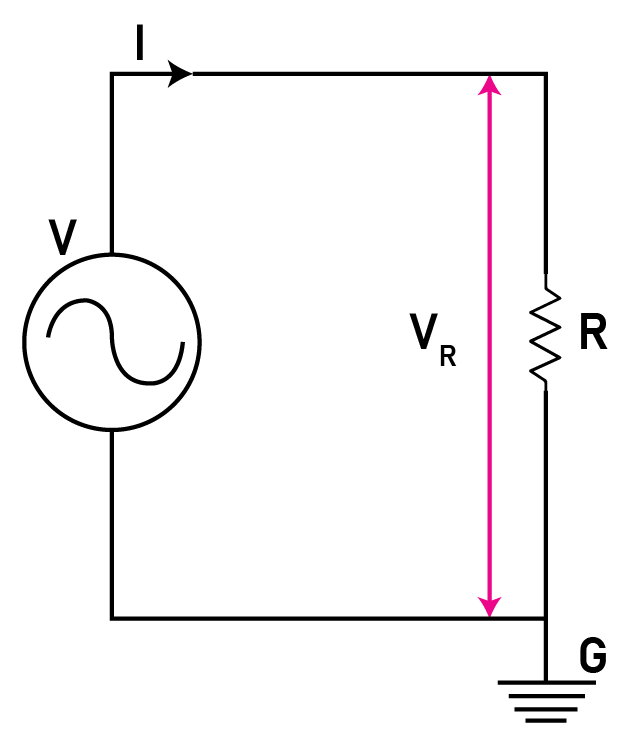
\includegraphics[scale = 0.9]{Images/Chapter-15/15.7}
    \caption{Resistor in A.C circuit.}
    \label{fig:15.7}
\end{figure}
\noindent We know that the instantaneous voltage ‘$V_{R}$’ across $R$ is
given by:
\begin{mybox}{red}{}
\begin{equation}\label{eq:15.11}
    V_{R} = V_{m} sin \omega t
\end{equation}
\end{mybox}
\noindent From Ohm’s law:
\begin{equation}\notag
    V_{R} = IR
\end{equation}
\begin{equation}\notag
    I= \frac{V_{R}}{R}
\end{equation}
Hence,
\begin{equation}\notag
    I = \frac{V_{m} sin \omega t}{R}
\end{equation}
Since,
\begin{equation}\notag
    \frac{V_{m}}{R} = I_{m}
\end{equation}
Hence,
\begin{mybox}{red}{}
\begin{equation}\label{eq:15.12}
    I = I_{m} sin \omega t
\end{equation}
\end{mybox}
\subsubsection{Waveform}
From equation \ref{eq:15.11} and \ref{eq:15.12}, it is obvious
that the waveform of voltage and
current is the same, as shown:
\begin{figure}[H]
    \centering
    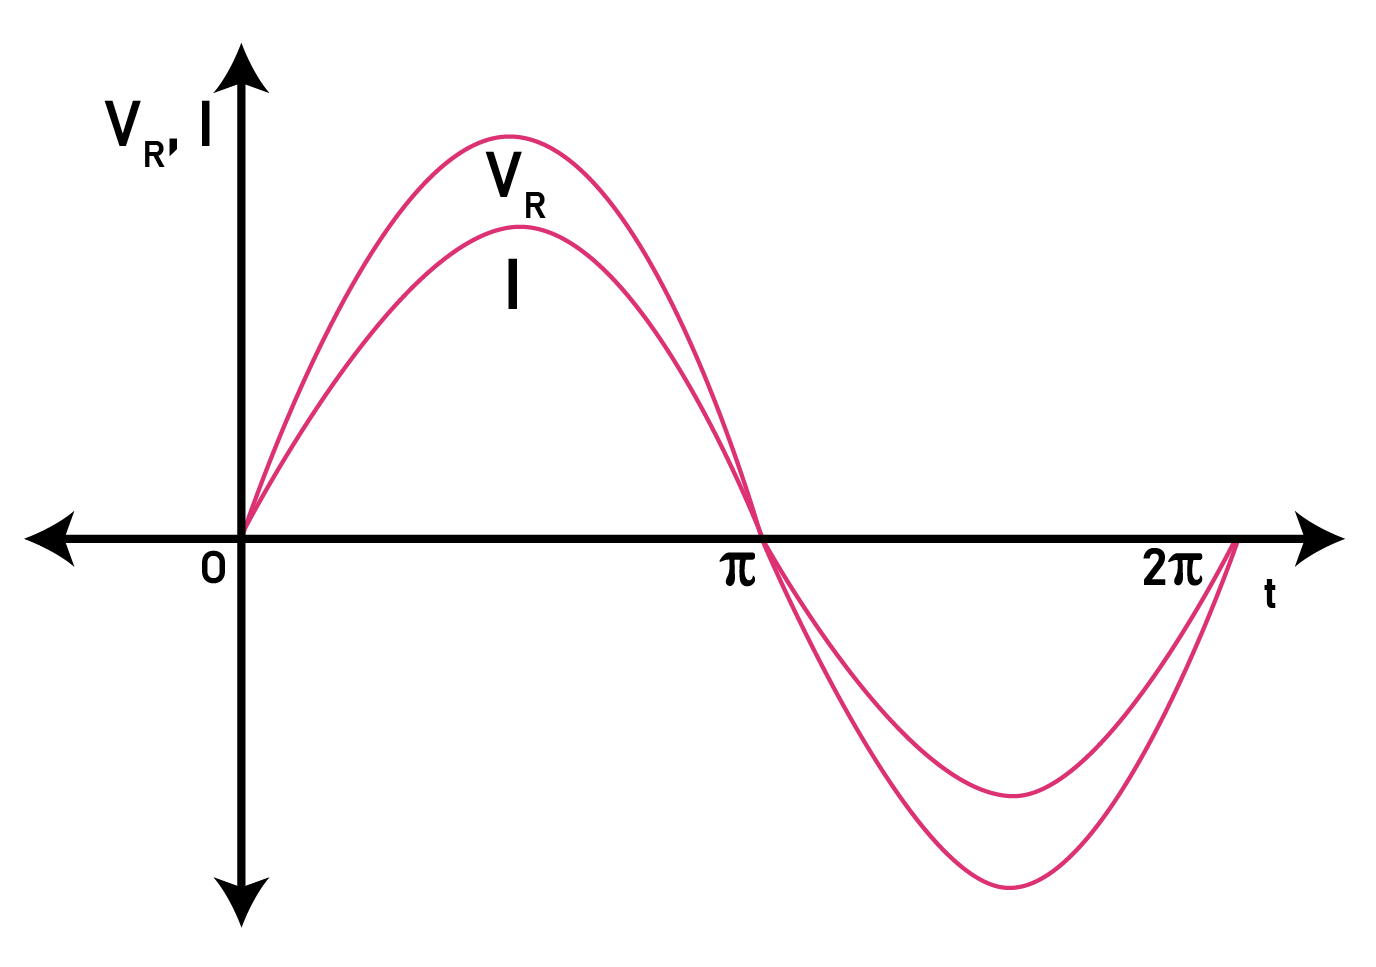
\includegraphics[scale = 0.8]{Images/Chapter-15/15.8}
    \caption{Voltage and current waveform for a pure resistive circuit.}
    \label{fig:15.8}
\end{figure}
\subsubsection{Phase}
The factor $\omega t$ (argument of sine) tells us about the starting point
of the waveform and is called phase of current or voltage.
From equations \ref{eq:15.11} and \ref{eq:15.12}, it is clear that
current and voltage are in phase, means reach the maximum 
and minimum value at the same time. So we can say that in a
purely resistive circuit, $I$ and $V$ are in phase.
\begin{figure}[H]
    \centering
    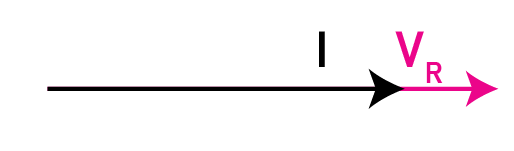
\includegraphics[]{Images/Chapter-15/15.9}
    \caption{Phasor for a pure resistive circuit.}
    \label{fig:15.9}
\end{figure}
\subsubsection{Power Loss}
The power curve for a pure resistive circuit is obtained from the
product of the corresponding instantaneous values of voltage and current.

Consider the figure \ref{fig:15.10} showing that power is always positive
where $I$ and $V$ are positive and zero for $I$ and $V$ zero.
It means that the voltage source is constantly delivering power
to the circuit, which is consumed by the circuit.
\begin{figure}[H]
    \centering
    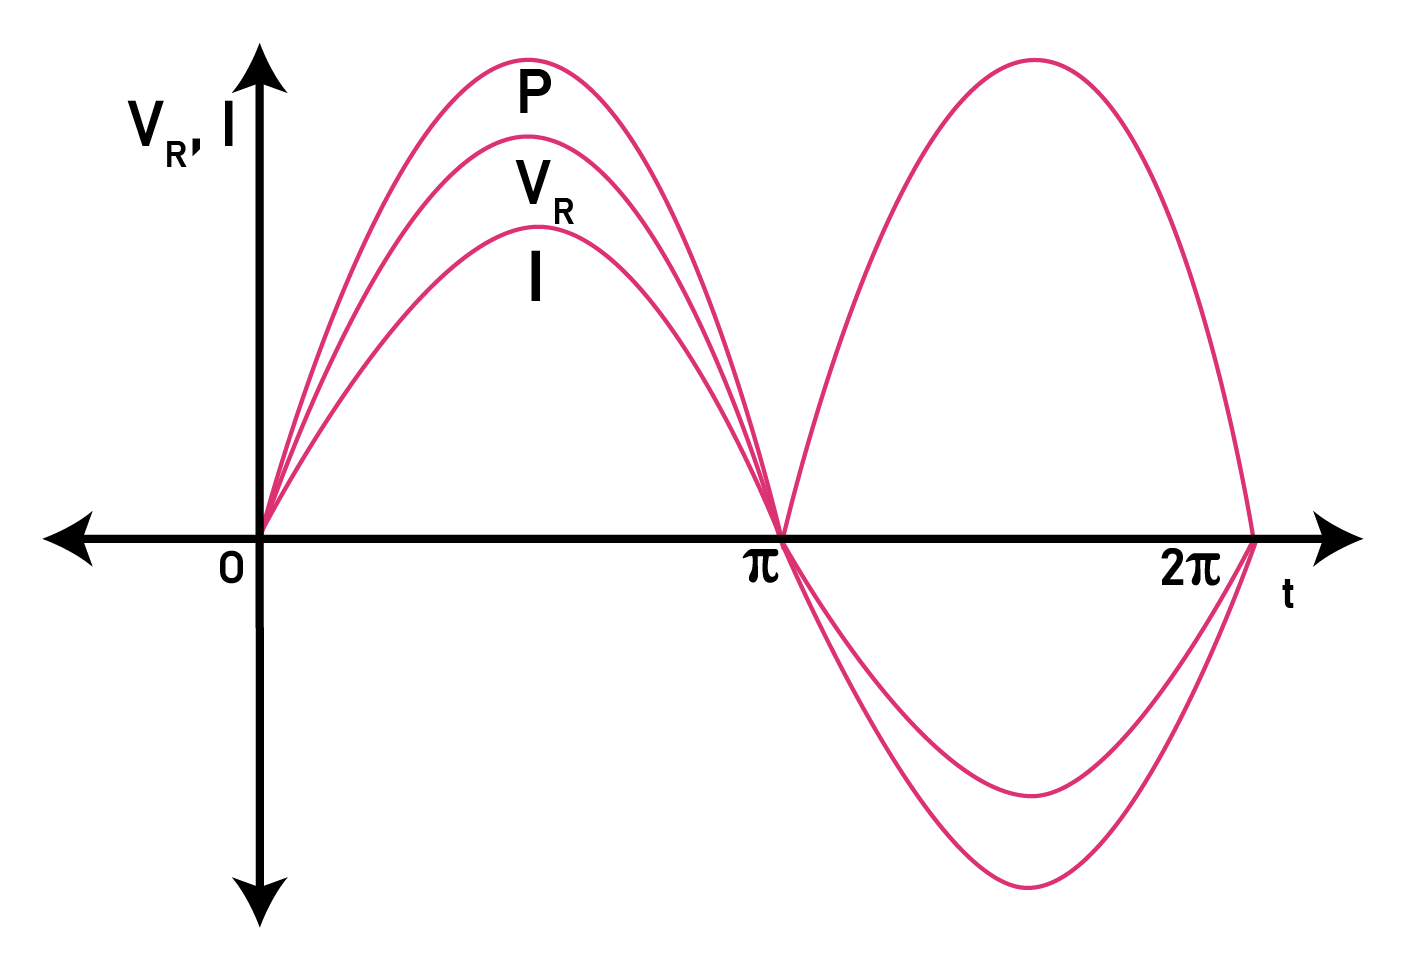
\includegraphics[scale = 0.8]{Images/Chapter-15/15.10}
    \caption{Power loss in a pure resistive circuit.}
    \label{fig:15.10}
\end{figure}
\subsubsection{Mathematical Form}
The average power dissipated in a resistor over the complete cycle of A.C is:
\begin{equation}\notag
    P_{avg} = <VI>
\end{equation}
\begin{equation}\notag
    P_{avg} = <V_{m} sin \omega t I_{m} sin \omega t>
\end{equation}
\begin{equation}\notag
    P_{avg} = V_{m} I_{m}  <sin^{2} \omega t>
\end{equation}
\begin{equation}\notag
    P_{avg} = \frac{V_{m} I_{m}}{2}
\end{equation}
\begin{mybox}{red}{}
    \begin{equation}\label{eq:15.13}
        P_{avg} = V_{rms} I_{rms}
    \end{equation}
\end{mybox}
\noindent So, the average value of power dissipated in a pure resistive
circuit is the product of rms values of voltage and current.
\subsection{Capacitor in an A.C Circuit:}
\subsubsection{Capacitor}
\textit{\textbf{``A device for storing electric charges and hence energy
is called capacitor."}}
\subsubsection{Capacitor in D.C Circuit}
If a D.C source is connected to a capacitor, the plates of the
capacitor quickly acquire equal and opposite charges and the
current in the circuit dies quickly. Afterwards, there is no
current in the circuit.
\subsubsection{Capacitor with A.C}
Let us consider a capacitor of capacitance $C$ connected in an A.C
circuit as shown in figure \ref{fig:15.11}.
\begin{figure}[H]
    \centering
    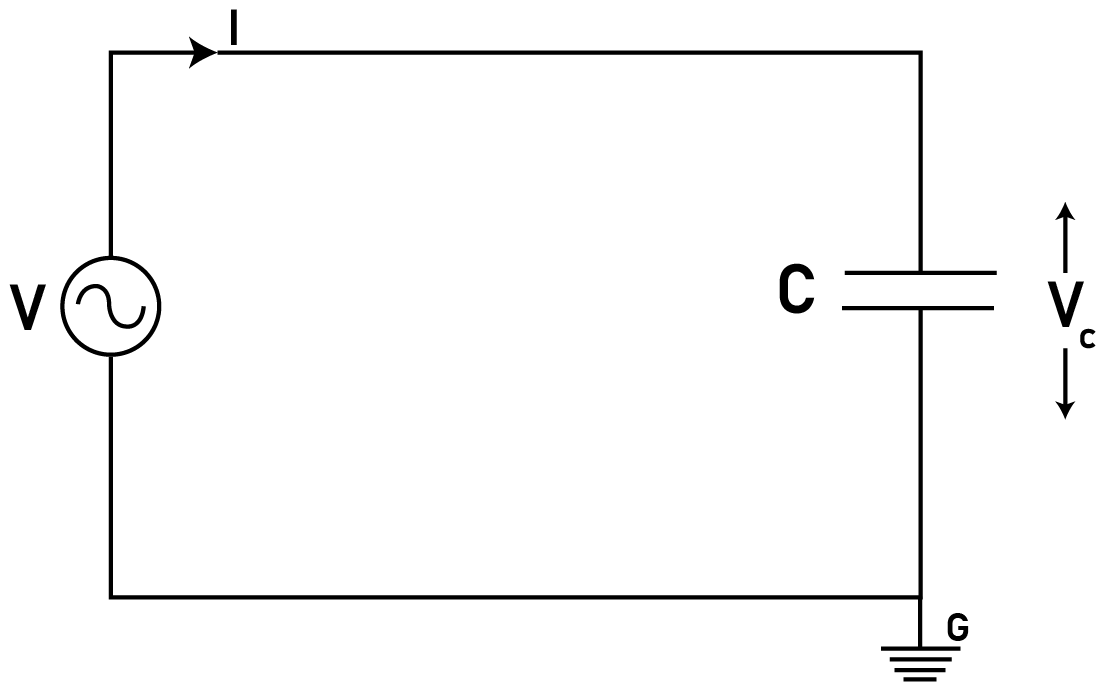
\includegraphics[scale = 0.8]{Images/Chapter-15/15.11}
    \caption{Capacitor in A.C circuit.}
    \label{fig:15.11}
\end{figure}
We are interested in discussing the voltage created across the plates
of capacitor and the current in the circuit. So when an A.C voltage
is first turned on, charge begins to flow and one plate acquires a
positive charge and the other a negative charge. Now, when the voltage
reverses itself, the current flows in opposite direction.
Thus we can say that an alternating voltage creates and AC in the circuit.

\subsubsection{Derivation}
As we know that the instantaneous voltage across the capacitor ‘$C$’ is given by:
\begin{equation}\notag
    V_{C} = V_{m} sin \omega t
\end{equation}
Also,
\begin{equation}\notag
   Q = CV_{C}
\end{equation}
Putting value of `$V_{C}$', we get:
\begin{equation}\notag
   Q = C V_{m} sin \omega t
\end{equation}
Take rate of change (derivative):
\begin{equation}\label{eq:15.14}
   \frac{dQ}{dt} = \frac{C V_{m} dsin \omega t}{dt}
\end{equation}
As $\frac{dQ}{dt} = I$ and $\frac{d}{dt}(sin\omega t) = \omega cos \omega t$,
hence equation \ref{eq:15.14} implies:
\begin{equation}\notag
   I = C V_{m} \omega cos \omega t
\end{equation}
If $\omega t=0$, current will be maximum i.e.
\begin{equation}\notag
   I_{m} = C V_{m} \omega 
\end{equation}
So,
\begin{mybox}{red}{}
    \begin{equation}\label{eq:15.15}
        I = I_{m} cos \omega t
    \end{equation}  
\end{mybox}
\noindent Equivalently,
\begin{mybox}{red}{}
\begin{equation}\label{eq:15.16}
    I = I_{m} sin(\omega t + \frac{\pi}{2})
\end{equation}
\end{mybox}
\subsubsection{Shape of the Graph}
The voltage varies with the sine of ‘$\omega t$’ and current as
cosine of ‘$\omega t$’ as shown:
\begin{figure}[H]
    \centering
    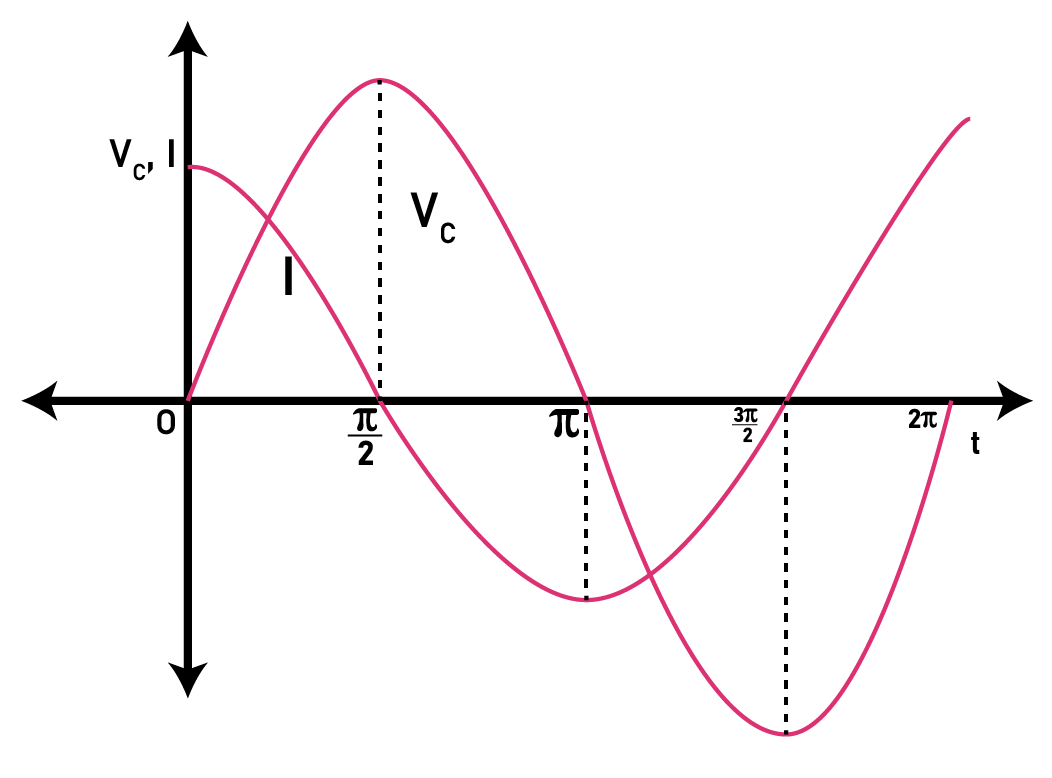
\includegraphics[]{Images/Chapter-15/15.12}
    \caption{Waveform of $V$ and $I$ for a pure capacitive circuit.}
    \label{fig:15.12}
\end{figure}
\subsubsection{Phase}
From equations \ref{eq:15.15} and \ref{eq:15.16},
it is obvious that the current is starting
($90^{\circ}$) quarter cycle before the voltage and
it is also clear from the graph. 
\newline
Let us explain:
\begin{enumerate}[label = $\square$]
    \item When $\omega t = 0^{\circ}$, $I=I_{m}$, $V_{C}=0$
    \item When $\omega t = 90^{\circ}$, $V_{C}=V_{m}$, $I=0$
    \item When $\omega t = 180^{\circ}$, $V_{C}=0$, $I=-I_{m}$
    \item When $\omega t = 270^{\circ}$, $V_{C}=-V_{m}$, $I = 0$
    \item When $\omega t =360^{\circ}$, $V_{C}=0$, $I=I_{m}$
\end{enumerate}
From the above data, it is concluded that current is flowing through
the circuit and reaches its maximum value yet no voltage is developed
across the plates of capacitor. When the voltage across the plates
reaches its maximum value, the current in the circuit ceases to zero.
Now, when the applied voltage direction is reversed, the current in
the circuit reverses its direction too. The current in the circuit
reaches its maximum value when the voltage across the plates becomes zero.
So all the time, \textit{\textbf{the current through the circuit is
leading the voltage by $90^{\circ}$ or $\frac{\pi}{2}\:rad$.}}

\subsubsection{Phasor Diagram}
\begin{figure}[H]
    \centering
    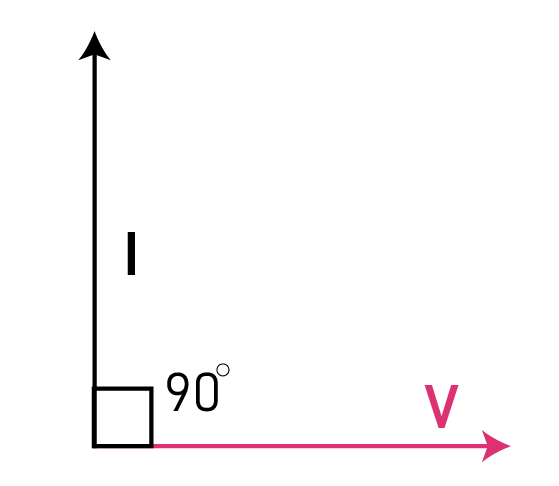
\includegraphics[]{Images/Chapter-15/15.13}
    \caption{Phasor Diagram for pure capacitive circuit.}
    \label{fig:15.13}
\end{figure}
\subsubsection{Reactance of a Capacitor}
In analogy with Ohm’s law, the ratio $\frac{V}{I}$ is the opposition to
the flow of current in A.C circuit. In case of a capacitor introduced
in the circuit, this ratio us called reactance
so as to distinguish from resistance and us defined as,
\textit{\textbf{``The capacitive reactance is the measure of opposition
offered by the capacitor to the flow of AC.”}}
It is denoted by $X_{c}$.
\subsubsection{Mathematical Form}
\begin{equation}\notag
    X_{c}=\frac{V_{m}}{I_{m}}
\end{equation}
Putting $I_{m} = CV_{m}\omega$, we get:
\begin{equation}\notag
    X_{c}=\frac{V_{m}}{CV_{m}\omega}
\end{equation}
\begin{mybox}{red}{}
\begin{equation}\label{eq:15.17}
    X_{c}=\frac{1}{\omega C}
\end{equation}
\begin{equation}\label{eq:15.18}
    X_{c}=\frac{1}{2 \pi fC}
\end{equation}
\end{mybox}
\noindent Hence for D.C, $f=0$, hence $X_{c} = \infty$. We can say
\textit{\textbf{``Capacitance offers infinite opposition to D.C."}}
For A.C, $X_{c}$ decreases as $f$ and $C$ increase.
Certain capacitors will have a large reactance at low frequency.
So the magnitude of the opposition offered by it will be large and
the current in the circuit will be small. On the other hand, at high
frequency, the reactance will be low and high frequency current through
the same capacitor will be large.

\subsubsection{Power Loss in a Capacitor}
  The instantaneous power is given by:
  \begin{equation}\notag
      P = IV
  \end{equation}
and Average power is given by:
  \begin{equation}\notag
    P_{avg} = V_{m}I_{m}< sin \omega t  cos \omega t>
\end{equation}
As $< sin \omega t  cos \omega t> = 0$, Hence:
\begin{mybox}{red}{}
\begin{equation}\notag
    P_{avg} = 0
\end{equation}
\end{mybox}
It means that average power dissipated in a pure capacitive
circuit is zero. Energy from the source is fed into the capacitor
where it is stored in the electric field between the plates.
As the field decreases, the energy returns to the source.
\textit{\textbf{Thus no power is dissipated in a pure capacitive circuit.}}
\subsubsection{Power Curve}
\begin{figure}[H]
    \centering
    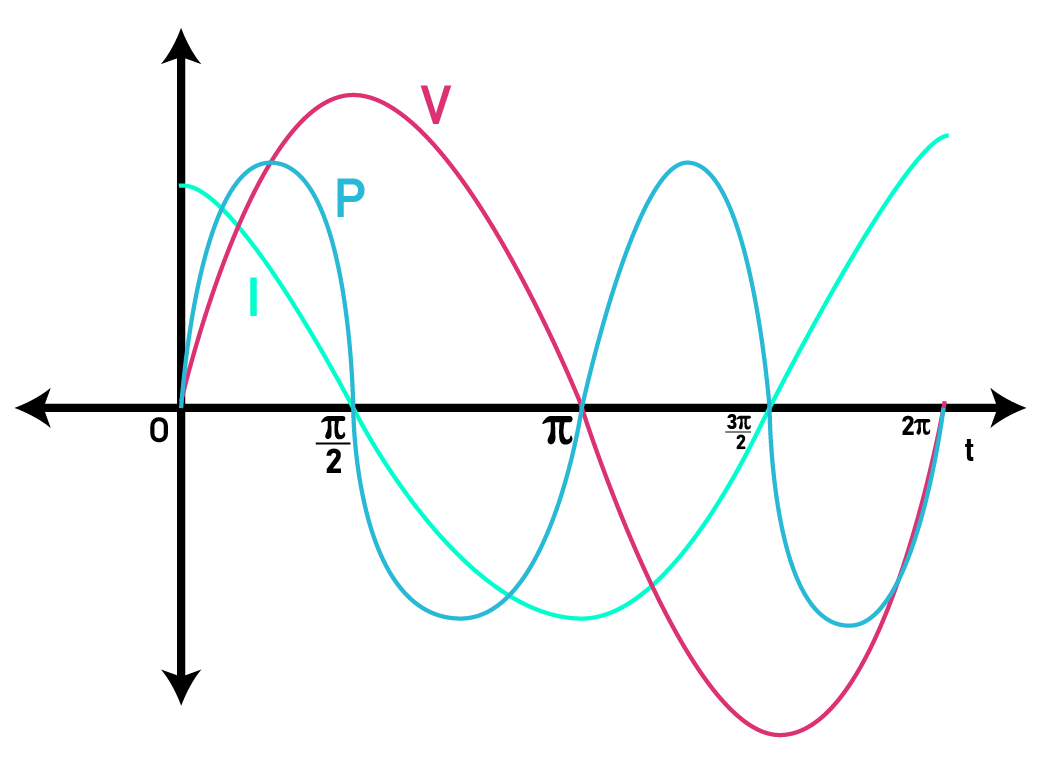
\includegraphics[]{Images/Chapter-15/15.14}
    \caption{Power curve for pure capacitive circuit.}
    \label{fig:15.14}
\end{figure}
From the figure \ref{fig:15.14}, it is clear that per cycle, as much the curve is
positive (the power is delivered to capacitor), by the same amount,
it is negative (power is delivered back to source). Positive power is
equal to the negative power, so power is absorbed by capacitor in one
cycle is zero.
\subsection{Inductor in an A.C Circuit}
\subsubsection{Inductor}
\textit{\textbf{``A coil wound from a thick wire so that it has a
large value of self-inductance ‘$L$’ and has a negligible resistance
is known as inductor."}} 
\subsubsection{Inductor with A.C}
Let us consider an inductor ‘$L$’ connected with an A.C source as shown:
   %figure
   
When an A.C voltage is applied across an inductor,
it must oppose the flow of current which is continuously changing,
therefore the current developed in the inductor lags behind
the applied voltage.
\subsubsection{Mathematical Derivation}
When a sinusoidal current `$I$' flows in time `$t$', then
a back emf is induced due to the inductance of the coil.
The back emf at each instant opposes the change in current
through the coil. As there is no drop in potential,
so the applied voltage has to overcome the back emf.
\begin{center}
    $Applied \ voltage=back \ emf$
\end{center}
As the current through the circuit is given by:
\begin{equation}\notag
    I = I_{m} sin \omega t
\end{equation}
This sinusoidally changing current sets up a back emf in the coil,
and is given by:
\begin{equation}\notag
    \mathcal{E}= L \frac{dI}{dt}
\end{equation}
To maintain a constant current, a constant voltage equal to back emf
must be applied i.e.
\begin{equation}\notag
    V = L \frac{dI}{dt}
\end{equation}
Putting value of I:
\begin{equation}\notag
    V = L \frac{d(I_{m}sin\omega t)}{dt}
\end{equation}
So,
\begin{equation}\notag
    V = L I_{m} \omega cos\omega t
\end{equation}
Writing $V_{m} = L I_{m} \omega$, we get:
\begin{mybox}{red}{}
\begin{equation}\label{eq:15.19}
    V = V_{m} cos \omega t
\end{equation}
Equivalently,
\begin{equation}\label{eq:15.20}
    V = V_{m} sin( \omega t + \frac{\pi}{2})
\end{equation}
\end{mybox}

\subsubsection{Shape of the Graph}
Both current and voltage are varying sinusoidally.
Current is varying with sine of ‘$\omega t$’ and voltage with
cosine of ‘$\omega t$’ as shown:
%figure

\subsubsection{Phase}
From the equations of voltage and current, it is clear that voltage leads the current by $\frac{\pi}{2}$ rad or 90\textsuperscript{$\circ$} or current lags behind the voltage by 90\textsuperscript{$\circ$}.
Let us explain:
\begin{enumerate}[label = $\square$]
    \item When $\omega t = 0^{\circ}$, $I=I_{m}(0) = 0$, $V_{L}=V_{m}(1) = V_{m}$
    \item When $\omega t = 90^{\circ}$, $V_{L}=0$, $I=I_{m}$
    \item When $\omega t = 180^{\circ}$, $V_{L}=V_{m}$, $I=0$
    \item When $\omega t = 270^{\circ}$, $V_{L}=0$, $I=I_{m}$
    \item When $\omega t =360^{\circ}$, $V_{L}=V_{m}$, $I=0$
\end{enumerate}

So from the above results, we can say that when voltage is applied to
the inductor, no current flows at once because of back emf.
The current reaches its maximum value when the voltage is zero. 
\textit{\textbf{All the time, the voltage through circuit is leading
the current by 90\textsuperscript{$\circ$} or $\frac{\pi}{2}$ rad.}}

\subsubsection{Phasor Diagram}
%%figure

\subsubsection{Inductive Reactance}
As from the pure inductive circuit voltage $V_{m}$ is given by:
\begin{equation}\label{eq:15.21}
    V_{m}=\omega LI_{m}
\end{equation}
From Ohm’s law:
\begin{equation}\label{eq:15.22}
    V_{m}= I_{m}R
\end{equation}
Comparing equations \ref{eq:15.21} and \ref{eq:15.22}:
\begin{equation}\notag
    \omega LI = IR
\end{equation}
Hence ,
\begin{equation}
    R = \omega L
\end{equation}
The factor here in replacement of ‘$R$’ in an inductive circuit is
called inductive reactance and is the measure
of opposition offered by the inductor to the flow of A.C. 
\newline
So, we can write:
\begin{mybox}{red}{}
\begin{equation}\label{eq:15.24}
    X_{L} = \omega L
\end{equation}
\end{mybox}
\paragraph{Unit:}
The unit for $X_{L}$ is same as for resistance (ohms).
\paragraph{Frequency Response:}
From equation \ref{eq:15.24}:
\begin{equation}\notag
    X_{L} = \omega L
\end{equation}
Putting $\omega = 2\pi f$:
\begin{equation}\notag
    X_{L} = 2\pi f L
\end{equation}
For D.C, $f=0$, hence,
\begin{equation}\notag
    X_{L}=0
\end{equation}
For A.C, \textit{\textbf{$X_{L}$ decreases as $f$
decreases and increases for increasing $f$.}}

\subsubsection{Power Dissipation}
The average power dissipated in an inductor over one cycle is :
\begin{equation}\notag
      P=IV
\end{equation}
\begin{equation}\notag
    P_{avg} = V_{m}I_{m}< sin \omega t  cos \omega t>
\end{equation}
\begin{mybox}{red}{}
\begin{equation}\notag
      P_{avg}=0
\end{equation}
\end{mybox}
So the average power in a pure inductive circuit over one whole cycle
is zero.
\subsubsection{Power Curve}
%figure
From the graph, we see that for first 90$\circ$ of the cycle,
both voltage and current are positive and the power dissipated is positive. Therefore, power flows from the source to the coil. Similarly, for the next 90$\circ$ of the cycle, power flows from the coil to the source. For next 90$\circ$, it is again positive and in last 90$\circ$, it is again negative. So over one cycle, the positive power is equal to the negative power.
So the resultant power over each cycle is zero.
Energy from the source is fed into the inductor where it is stored
in the magnetic field. As the field decreases, the energy returns
to the source. Thus no power is dissipated in the pure inductive circuit.
\section{Choke Coil}
\textit{\textbf{“It is an inductor having high reactance and
low resistance used for reducing high frequency component of alternating
signal.”}}
\subsection*{Explanation}
 It consists of a thick copper wire wounded closely in a large
 number of turns over a soft iron laminated core. This makes the
 inductance ‘$L$’ of the coil very large and resistance very small.
 Thus it consumes a little power.
  
 In general, a choke is used to prevent electrical signals along
 undesired paths. The choke is used as a filter in power supply to
 prevent ripple. It also prevents unwanted signals to enter other parts
 of the circuits e.g radio frequency choke (RFC) prevents radio frequency
 signals from entering audio frequency circuits, thus undesired signals
 and noise can be attenuated.
\section{Impedance}
\textit{\textbf{“It is the combined opposition offered by the
circuit elements to the alternating current.”}}
\subsection*{Symbol}
  It is symbolized as `$Z$'. 
\subsection*{Explanation}
We know that the resistance `$R$' offers opposition to the flow of
D.C as well as A.C. On the other hand, inductor does not oppose D.C
and capacitor has an infinite opposition to D.C.
 
In case of A.C, an inductance ‘$L$’ or a capacitance ‘$C$’ offers
finite opposition which is measured by the reactances ‘$X_{L}$’
and ‘$X_{C}$’ respectively. If an A.C circuit consists of a resistance
‘$R$’, an inductance ‘$L$’ and a capacitance ‘$C$’, the combined
opposition of these elements will be called as impedance of the circuit.
\subsection*{Mathematical Form}
Impedance is the ratio of rms values of applied voltage and alternating
current.
\begin{mybox}{red}{}
\begin{equation}\label{eq:15.25}
    Z=\frac{V_{rms}}{I_{rms}}
\end{equation}{}
\end{mybox}
\subsection*{Unit}
Similar to resistance, impedance is the resistance so it is also expressed
in ohms.
\section{RL-Series Circuit}
\textit{\textbf{“The circuit in which resistor ‘$R$’ and inductor
‘$L$’ are connected in series.”}}
\subsection*{Circuit Diagram}
%figure
\subsection*{Explanation}
For RL circuit, we are interested in finding the impedance, current and
phase angle between the current and voltage. As there is same current
through each component, so we consider the current as the reference phasor.
Now to understand the RL circuit, we know in resistor, voltage and current
are in phase. So, $V_{R}$ vector will be parallel to $I$. Also, we know
that the potential difference across inductor ‘$V_{L}$’ leads $I$ by 90
degrees. Therefore phasor $V_{L}$ is in upward direction
and $V_{R}$ will be parallel to $I$. The resultant $V$ will be the
vector sum of $V_{R}$ and $V_{L}$.

\subsection*{Mathematical Derivation}
To calculate the current, impedance and phase angle, let us consider the
above statements in a diagram. The vector $V_{R}$ is in
phase with $I$ as represented by magnitude and direction by phasor
$\vec{OP}$. The voltage $V_{L}$ leads the current by 90 degrees and is
represented in magnitude and direction by phasor $\vec{PM}$ as shown:
%figure

$\phi$ is the angle between $V_{L}$ and $V_{R}$. Now we calculate:

\subsubsection{Current(I)}
Applying Pythagoras Theorem:
\begin{equation}\notag
    V^{2}=V_{L}^{2} + V_{R}^{2}
\end{equation}
Put $V_{R}=IR$ and $V_{L}=IX_{L}$, we get:
\begin{equation}\notag
    V^{2}=I^{2}X_{L}^{2} + I^{2}R^{2}
\end{equation}
\begin{equation}\notag
    V^{2}=I^{2} (X_{L}^{2} + R^{2})
\end{equation}
\begin{equation}\notag
    V=I \sqrt{ (X_{L}^{2} + R^{2})}
\end{equation}
Hence,
\begin{mybox}{red}{}
\begin{equation}\label{eq:15.26}
    I=\frac{V}{\sqrt{ (X_{L}^{2} + R^{2})}}
\end{equation}
\end{mybox}
\noindent This is the equation for the current.
\subsubsection{Impedance}
From the definition of Impedance:
\begin{equation}\notag
    Z = \frac{V}{I}
\end{equation}
Put value of I from equation \ref{eq:15.26}:
\begin{mybox}{red}{}
\begin{equation}
    Z = \sqrt{ (X_{L}^{2} + R^{2})}
\end{equation}
\end{mybox}
The quantity $\sqrt{X_{L}^{2} + R^{2}}$ is the opposition offered
by the RL circuit components to the current flow and is called
impedance of the circuit.
\subsubsection{Phase Angle}
From the diagram, the current $I$ (which is in the horizontal x-direction;
the reference direction) lags behind the voltage $V$ of the circuit
by $\phi$, which is less than $90^{\circ}$.

From figure:
\begin{equation}\notag
    tan \phi =\frac{V_{L}}{V_{R}}
\end{equation}
Put $V_{R}=IR$ and $V_{L}=IX_{L}$:
\begin{equation}\notag
    tan \phi =\frac{IX_{L}}{IR}
\end{equation}
\begin{mybox}{red}{}
\begin{equation}\label{eq:15.28}
      \phi =tan^{-1}\frac{X_{L}}{R}
\end{equation}
\end{mybox}
\noindent From equation \ref{eq:15.28}, it is also clear that:
\begin{enumerate}[label = (\roman*)]
    \item When $\phi\rightarrow 90^{\circ}$, $\omega\rightarrow\infty$.
    \item When $\phi\rightarrow 0^{\circ}$, $\omega$ $\rightarrow 0$.
\end{enumerate}
It means that RL-series A.C circuit will behave like a pure inductive
circuit for very high frequency and pure resistive circuit for very low
frequency.
\subsection*{Power in RL Circuit}
To calculate the power in RL circuit, let us write equation for the circuit
current $I$ and voltage $V$.
As,
\begin{equation}\notag
    I = I_{m} sin (\omega t - \phi)
\end{equation}
And
\begin{equation}\notag
    V = V_{m} sin \omega t
\end{equation}
It means that voltage leads the current by $\phi$.Now,
\begin{equation}\notag
   P_{avg}=<IV>
\end{equation}
\begin{equation}\notag
   P_{avg}=<I_{m} sin (\omega t - \phi)  V_{m} sin \omega t >
\end{equation}
\begin{equation}\notag
   P_{avg}=I_{m}  V_{m}<  sin \omega t sin (\omega t - \phi)  >
\end{equation}
Use formula from trigonometry:
\begin{equation}\notag
   sin(a-b)=sina cosb-cosa sinb
\end{equation}
So, we can write $P_{avg}$ as:
\begin{equation}\notag
   P_{avg}=I_{m}  V_{m}<  sin \omega t (sin \omega t cos \phi - cos \omega t sin \phi )  >
\end{equation}
\begin{equation}\notag
   P_{avg}=I_{m}  V_{m}<  sin^{2} \omega t cos \phi - cos \omega t sin\omega t sin \phi )  >
\end{equation}
Pulling constants out of average:
\begin{equation}\notag
   P_{avg}=I_{m}  V_{m}(  cos \phi <sin^{2} \omega t> -sin \phi< cos \omega t sin\omega t > )  
\end{equation}
Since $<sin^{2} \omega t> = \frac{1}{2}$ and $<cos \omega t sin\omega t>=0$,
Hence,
\begin{equation}\notag
   P_{avg} =I_{m}  V_{m}(\frac{cos \phi}{2}-0)
\end{equation}
\begin{equation}\notag
   P_{avg} = \frac{I_{m}  V_{m} cos \phi}{2}
\end{equation}
\begin{mybox}{red}{}
\begin{equation}
   P_{avg} = I V cos \phi
\end{equation}
\end{mybox}
\begin{mybox}{green}{}
\subsection*{\note{}Note}
\begin{enumerate}[label = $\square$]
\item We are writing $I$ and $V$, it is understood that the
values we will take into account are rms values of voltage and current.
\item It is also important that in analogy to D.C where
$P = I^{2}R$, here average power is equal to $I_{rms}^{2}R$,
normally written as $I^{2}R$ in A.C circuits.
\end{enumerate}
\end{mybox}
\subsubsection{Power Curve}
The power curve for a phase angle of 30 degrees is shown as:
%figure

\paragraph{Note:}
As $tan \phi = \frac{X_{L}}{R}$, when $\phi$ is large i.e greater the
phase angle, larger will be the reactance compared to the resistance
and less will be the power consumption.

\section{RC Series A.C Circuit}
\textit{\textbf{“The circuit in which resistor $R$, capacitor $C$ are
connected in series with an alternating voltage.”}}
\subsection*{Circuit Diagram}
Let us consider a capacitor $C$ and resistor $R$ connected in series
with an alternating voltage $V$ as shown:
%figure

\subsection*{Explanation}
As the same current flows through each component, so will consider
current to be our reference phasor. $V_{R}$ is the voltage across the
resistor and $V_{C}$ is the voltage across the capacitor.
As in resistor, voltage and current are in phase, so $V_{R}$ must be
parallel to $I$. Also we know that the potential difference across $C$
is $V_{C}$ and it lags behind $I$ by 90 degrees. Hence the vector
$V_{C}$ must be in downward direction. The vector sum of $V_{C}$
and $V_{R}$ equals the potential difference applied $V$.

\subsection*{Mathematical Derivation}
To calculate current, impedance and phase angle, we will draw a diagram
based on above explanation.
\subsubsection{Current}
Applying Pythagoras Theorem:
\begin{equation}\notag
    V^{2}=V_{C}^{2} + V_{R}^{2}
\end{equation}
Put $V_{R}= IR$ and $V_{C}=IX_{C}$:
\begin{equation}\notag
    V^{2}=I^{2}X_{C}^{2} + I^{2}R^{2}
\end{equation}
\begin{equation}\notag
    V^{2}=I^{2} (X_{C}^{2} + R^{2})
\end{equation}
\begin{equation}\notag
    V=I \sqrt{ (X_{C}^{2} + R^{2})}
\end{equation}
Hence,
\begin{mybox}{red}{}
\begin{equation}\label{eq:15.30}
    I=\frac{V}{\sqrt{ (X_{C}^{2} + R^{2})}}
\end{equation}
\end{mybox}
This is the equation for the current.
\subsubsection{Impedance}
From the definition of impedance :
\begin{equation}\notag
    Z = \frac{V}{I}
\end{equation}
Put value of $I$ from equation \ref{eq:15.30}:
\begin{mybox}{red}{}
\begin{equation}\label{eq:15.31}
    Z = \sqrt{ (X_{C}^{2} + R^{2})}
\end{equation}
\end{mybox}
The quantity $\sqrt{X_{C}^{2} + R^{2}}$ is the opposition offered by
the RC circuit components to the current flow and is called impedance
of the circuit.
\subsubsection{Phase Angle}
From the diagram, the current $I$(which is in the horizontal
x-direction; the reference direction) leads the voltage $V$ of the
circuit by $\phi$, which is less than $90^{\circ}$.
From figure:
\begin{equation}\notag
    tan \phi =\frac{V_{C}}{V_{R}}
\end{equation}
Put $V_{R}=IR$ and $V_{C}=IX_{C}$:
\begin{equation}\notag
    tan \phi =\frac{IX_{C}}{IR}
\end{equation}
\begin{mybox}{red}{}
\begin{equation}\label{eq:15.32}
    \phi =tan^{-1}\frac{X_{C}}{R}
\end{equation}
\end{mybox}
\noindent From equation \ref{eq:15.31}, it is also clear that:
\begin{enumerate}[label = (\roman*)]
    \item When $\phi\rightarrow 0^{\circ}$, $\omega\rightarrow\infty$.
    \item When $\phi\rightarrow 90^{\circ}$, $\omega$ $\rightarrow 0$.
\end{enumerate}
It means that RL-series A.C circuit will behave like a pure inductive
circuit for very high frequency and pure resistive circuit for very
low frequency.

\subsection*{Power in RC Circuit}
To calculate the power in RC circuit,
let us write equation for the circuit current $I$ and voltage $V$.
As,
\begin{equation}\notag
    I = I_{m} sin (\omega t - \phi)
\end{equation}
And
\begin{equation}\notag
    V = V_{m} sin \omega t
\end{equation}
It means that voltage leads the current by $\phi$. Now,
\begin{equation}\notag
   P_{avg}=<IV>
\end{equation}
\begin{equation}\notag
   P_{avg}=<I_{m} sin (\omega t - \phi)  V_{m} sin \omega t >
\end{equation}
\begin{equation}\notag
   P_{avg}=I_{m}  V_{m}<  sin \omega t sin (\omega t - \phi)  >
\end{equation}
Use formula from trigonometry:
\begin{equation}\notag
   sin(a-b)=sina cosb-cosa sinb
\end{equation}
So, $P_{avg}$ can be written as:
\begin{equation}\notag
   P_{avg}=I_{m}  V_{m}<  sin \omega t (sin \omega t cos \phi - cos \omega t sin \phi )  >
\end{equation}
\begin{equation}\notag
   P_{avg}=I_{m}  V_{m}<  sin^{2} \omega t cos \phi - cos \omega t sin\omega t sin \phi )  >
\end{equation}
Pulling constants out of average:
\begin{equation}\notag
   P_{avg}=I_{m}  V_{m}(  cos \phi <sin^{2} \omega t> -sin \phi< cos \omega t sin\omega t > )  
\end{equation}
Since $<sin^{2} \omega t = \frac{1}{2}>$ and $<cos \omega t sin\omega t>=0$,
Hence:
\begin{equation}\notag
   P_{avg} =I_{m}  V_{m}(\frac{cos \phi}{2}-0)
\end{equation}
\begin{equation}\notag
   P_{avg} = \frac{I_{m}  V_{m} cos \phi}{2}
\end{equation}
\begin{mybox}{red}{}
\begin{equation}\label{eq:15.33}
   P_{avg} = I V cos \phi
\end{equation}
\end{mybox}
\begin{mybox}{green}{}
\subsubsection{Note}
In case of R.C circuit, the phase angle $\phi$ is in clockwise
direction because $V_{C}$ lies along negative y-axis. Some
authors do derivations by writing $V_{C}$ as $-V_{C}$  and hence
$\phi$ negative, which is also an approach. 
\end{mybox}
\section{RLC Series A.C Circuit}
\textit{\textbf{“The circuit containing resistor, inductor and
capacitor in series with an A.C source is called RLC series A.C circuit.”}}
\subsection{Explanation}
Let us consider an inductor $L$, resistor $R$ and capacitor $C$
connected with an A.C source as shown:
%figure
The purpose is to find the current, impedance and the phase angle of the
voltage with current.  find the required quantities, we must draw the
phasor diagram for the circuit. We know that in series the current in
all the circuit elements is same, therefore, it is taken as the
reference phasor and is drawn horizontally directed to the right as shown:
%figure   
   
Also we know that $V_{R}$  is in phase with $I$. The
voltage $V_{L}$ is leads $I$ by 90 degrees,
whereas $V_{C}$ lags behind the $I$ by 90 degrees i.e $V_{L}$ and
$V_{C}$ are out of phase by $180^{\circ}$.   
Now, there are two possibilities:
\begin{enumerate}[label = (\roman*)]
    \item If $V_{L}$ is greater than $V_{C}$,
    the resultant $V_{L}-V_{C}$ is in the direction of $V_{L}$.
    \item If $V_{C}$ is greater than $V_{C}$, the resultant $V_{L}-V_{C}$
    is in the direction of $V\textsubscript{C}$.
\end{enumerate}
It is shown as:
%figure
Now we discuss:
\subsubsection*{Current}
From either of Diagram, applying Pythagoras Theorem:
\begin{equation}\notag
    V^{2}=(V_{C}-V_{L})^{2} + V_{R}^{2}
\end{equation}
Since $(a-b)^{2}=(b-a)^2$, Hence,
\begin{equation}\notag
    V^{2}=(V_{L}-V_{C})^{2} + V_{R}^{2}
\end{equation}
Putting $V_{R}=IR$, $V_{C}=IX_{C}$ and
$V_{L}=IX_{L}$, we get:
\begin{equation}\notag
    V^{2}=I^{2}(X_{L}^{2}-X_{C}^{2}) + I^{2}R^{2}
\end{equation}
\begin{equation}\notag
    V^{2}=I^{2} ((X_{L}^{2}-X_{C}^{2}) + R^{2})
\end{equation}
\begin{equation}\notag
    V=I \sqrt{ ((X_{L}^{2}-X_{C}^{2}) + R^{2})}
\end{equation}
Hence,
\begin{mybox}{red}{}
\begin{equation}\label{eq:15.34}
    I=\frac{V}{\sqrt{ (X_{L}^{2}-X_{C}^{2}) + R^{2})}}
\end{equation}
\end{mybox}
\noindent This is the equation for the current.
\subsubsection*{Impedance}
From the definition of Impedance:
\begin{equation}\notag
    Z = \frac{V}{I}
\end{equation}
Put value of $I$ from equation \ref{eq:15.33}:
\begin{mybox}{red}{}
    \begin{equation}\label{eq:15.35}
        Z = \sqrt{ ((X_{L}^{2}-X_{C}^{2}) + R^{2})}
    \end{equation} 
\end{mybox}
\noindent The quantity $\sqrt{ (X_{L}^{2}-X_{C}^{2}) + R^{2})}$ is the
opposition offered by the RC circuit components to the current flow
and is called impedance of the circuit.
\subsubsection{Phase Angle}
From figure:
\begin{equation}\notag
    tan \phi =\frac{V_{L}-V{C}}{V_{R}}
\end{equation}
Put $V_{R}=IR, V_{L}=IX_{L}$ and $V_{C}=IX_{C}$:
\begin{mybox}{red}{}
\begin{equation}\label{eq:15.36}
    \phi =tan^{-1}\frac{X_{L}-X_{C}}{R}
\end{equation}
\end{mybox}
\subsection*{Impedance Triangle}
In analogy with phasor diagram, the impedance diagram is shown as:
%figure
\subsection*{Power Factor}
As power factor is given by:
\begin{mybox}{red}{}
\begin{equation}\label{eq:15.37}
    cos \phi = \frac{V_{R}}{V} = \frac{R}{Z}
\end{equation}
\end{mybox}
\subsection*{Power Dissipation}
Using formula:
\begin{mybox}{red}{}
\begin{equation}\label{eq:15.38}
    P_{avg} =I V cos \phi
\end{equation}
\end{mybox}
\noindent Now, we discuss some cases:
\paragraph{Case 1:}
The quantity $X_{L}-X_{C}$ is called
the reactance of the circuit. When $X_{L}-X_{C}$ is positive, i.e.
$X_{L}>X_{C}$, phase angle $\phi$ is positive and the circuit will
be inductive. In other words, the circuit current $I$ will lag behind
the voltage $V$ by $\phi$.
\paragraph{Case 2:}
When $X_{L}$-$X_{C}$ is negative, i.e. $X_{L}>X_{C}$, phase angle
$\phi$ is negative and the circuit is capacitive. That is to say that
circuit current $I$ leads the applied voltage by $\phi$.
\subsubsection{Case 3}
When $X_{L}-X_{C}=0$, i.e. $X_{L}=X_{C}$, the circuit is purely resistive.
In other words, circuit current $I$ and applied voltage $V$ will be in
phase i.e. $\phi=0^{\circ}$, the power factor will be unity.
\section{Series Resonance A.C Circuits}
\subsection*{Definition}
\textit{\textbf{“The situation in which the current in the circuit is
maximized is called electrical resonance.”}}
\begin{center}
    OR
\end{center}
\textit{\textbf{“The situation in which the inductive reactance is
equal to the capacitive reactance.”}}
\subsection*{Explanation}
In the impedance equation, along with the equations for the inductive and
capacitive reactances, we see that impedance has a rather complicated
dependence on frequency. As,
\begin{equation}\label{eq:15.39}
    Z = \sqrt{ ((X_{L}^{2}-X_{C}^{2}) + R^{2})}
\end{equation}
And
\begin{equation}\label{eq:15.40}
   I = \frac{V}{Z}
\end{equation}
Now, the frequency of circuit can be set so that the capacitive reactance
equals the inductive reactance i.e $X_{L}=X_{C}$ then according to equation
\ref{eq:15.39}, $Z$ will be equal to $R$ and by equation \ref{eq:15.40},
$I$ will be maximum. This condition is called resonance and is electrical
analogue to resonance in harmonic oscillators such as swinging pendulum of
a mass at the end of spring.
\subsubsection{Resonance Frequency}
As we know that at resonance,
\begin{center}
    $X_{L}=X_{C}$
\end{center}
Put $X_{L}=\omega L$ and $X_{C} = \frac{1}{\omega C}$:
\begin{equation}\notag
    \frac{1}{\omega C} = \omega L
\end{equation}
\begin{equation}\notag
    \omega^{2} = \frac{1}{LC}
\end{equation}
\begin{mybox}{red}{}
\begin{equation}\label{eq:15.41}
    \omega = \frac{1}{\sqrt{LC}}
\end{equation}
\begin{equation}\label{eq:15.42}
    f_{r} = \frac{1}{2\pi\sqrt{LC}}
\end{equation}
\end{mybox}
\noindent This is known as resonance frequency for a given $L$ and $C$.
\section{Electromagnetic Radiations}
Electromagnetic radiations such as infrared are different from each other
due to their properties. But they have some features in common such as
electric field and magnetic field. Therefore it can be described in
terms of electric and magnetic fields, and they all travel through
vacuum with the same speed (the speed of light).

Fundamentally these radiations are different only in wavelength or
frequency. The names given to them in figure below shows various regions
of the spectrum along with given names. There are no gaps in the spectrum,
nor their sharp boundaries between the various categories (certain regions
of spectrum are assigned by law for commercial or other uses such as T.V,
A.M, F.M broadcasting).

Let us consider some of these types of electromagnetic radiation in more
details: 
\subsection{Light}
The visible region of spectrum, most familiar to us, is the
electromagnetic radiation emitted by sun. The wavelength of light
ranges from about 400 nm (violet) to about 700 nm (red). Light is
often emitted when the outer (or valence) electrons in atoms change
their state of motion: for this reason, such transitions in the state
of the electron are called optical transitions. The color of the light
tells us something about the atoms or the object from which it was emitted. The study of the light emitted from the Sun and from distant stars gives information about their composition.
\subsection{Infrared}
Infrared radiation, which has wavelength stronger than the visible
(from 0.7 m to about 1 mm), is commonly emitted by atoms or molecules
when they change their rotational or vibrational motion.
Infrared radiation is an important means of heat transfer and is
sometimes called heat radiation. The warmth you feel when you place
your hand near a glowing light bulb is primarily a result of the infrared
radiation emitted from the bulb.

All Objects emit electromagnetic radiation (thermal radiation) because
of their temperature. Objects of temperatures ranges from  3K to 3000K
emit their most intense thermal radiation in the infrared region of the
spectrum.
          
A remote control is a component of an electronics device, most commonly a
television set, DVD player and home theater systems originally used for
operating the device wirelessly from a short line-of-sight distance.
The main technology used in home remote controls is infrared light.
The signal between a remote control handset and the device it controls
consists of pulses of infrared light, which is invisible to the human eye.
Infrared radiation is also used for cooking the surface of food
(the interior is then heated by convection and conduction).
\subsection{Microwaves}
Microwaves can be regarded as short radio waves, with typical wavelengths
in the range 1mm to 1m. They are commonly produced by electromagnetic
oscillators in electric circuits, as in the case of microwave ovens.
Microwaves are often used to transmit telephone conversations.
Figure shows a microwaves station that serves to relay telephone calls.
Microwaves also reach us from extraterrestrial sources.

Neutral hydrogen atoms, which populace the regions between the stars in
our galaxy, are common extraterrestrial source of Microwaves emitting
radiation with a wavelength of 21cm.
\subsection{Radio Waves}
Radio waves have wavelengths longer than 1 m. They are  produced from
terrestrial sources through electrons oscillating in wires of electric
circuits. By carefully choosing the geometry of these circuits, as in
an-antenna, we can control the distribution in space of the emitted
radiation (if the antenna acts as a transmitter) or the sensitivity
of the detector (if the antenna acts as a receiver). Traveling outward
at the speed of light, the expanding of TV signals transmitted on Earth. 

Radio waves reach us from extraterrestrial sources, the sun being a major
source that often interferes with radio or TV reception on Earth. Mapping
the radio emissions from extraterrestrial sources, known as radio
astronomy, has provided information about the universe that is often
not obtainable using optical telescopes.
\subsection{Ultraviolet}
The radiations of wavelengths shorter than the visible begin with
the ultraviolet (lnm to which can be produced in atomic transitions
of the outer- electrons as well as in radiation from thermal sources
such as the Sun. Because our atmosphere absorbs strongly at ultraviolet
wavelengths, little of this radiation from the Sun reaches the ground.
However, the principal agent of this absorption is atmospheric ozone,
which has been depleted in recent years as a result of chemical reactions
with fluorocarbons released from aerosol sprays, causes common sun burn
but long-term exposure can lead to more serious effects, including skin
cancer. 
\subsubsection{Ultraviolet Lamp(UV light)}
A lamp producing ultraviolet(UV) radiation emitted through clear,
pre-filtered , particle free water. This UV light is extremely effective
in killing and eliminating bacteria, yeasts, viruses, molds and other
harmful organisms known to man. It is used in industry and hospitals to
treat water. It is also used as a post disinfecting method for residential
water treatment. 
\subsection{X-rays}
X-rays (typical wavelengths 0.01 nm to 10 nm) can be produced with
discrete wavelengths In individual transitions among the inner
(most tightly bound) electrons Of an atom, and they can also be produced
when charged particles (such as electrons) are decelerated.
X rays can easily penetrate soft tissue but are stopped by bone and other
solid matter; for this reason they have found wide use in medical diagnosis.
\subsection{Gamma rays}
Gamma rays are electromagnetic radiations with the shortest wavelengths
less than 10 pm. They are the most penetrating of electromagnetic
radiations, and exposure to intense gamma radiation can have a harmful
effect on the human body. These radiations can be emitted in transitions
of an atomic nucleus from one state to another and can also occur in the
decays of certain elementary particles. For example, a neutral ion can
decay into two gamma rays according to
\begin{equation}\notag
    \pi^{0} = \gamma + \gamma
\end{equation}
